%	$Id$
% Internal documentation for slide modeling in grdseamount
% Paul Wessel, November 16, 2016.
\documentclass[12pt,letterpaper,margin=0.5in]{report}
\usepackage{times}
\usepackage{graphicx}
\usepackage{breqn}
\usepackage[margin=0.5in]{geometry}
\usepackage{lscape}
\textheight = 9 in
\topmargin = -1 in
\begin{document}

\section{Model curve for a landslide in grdseamount}

\begin{figure}[h!]
  \centering
  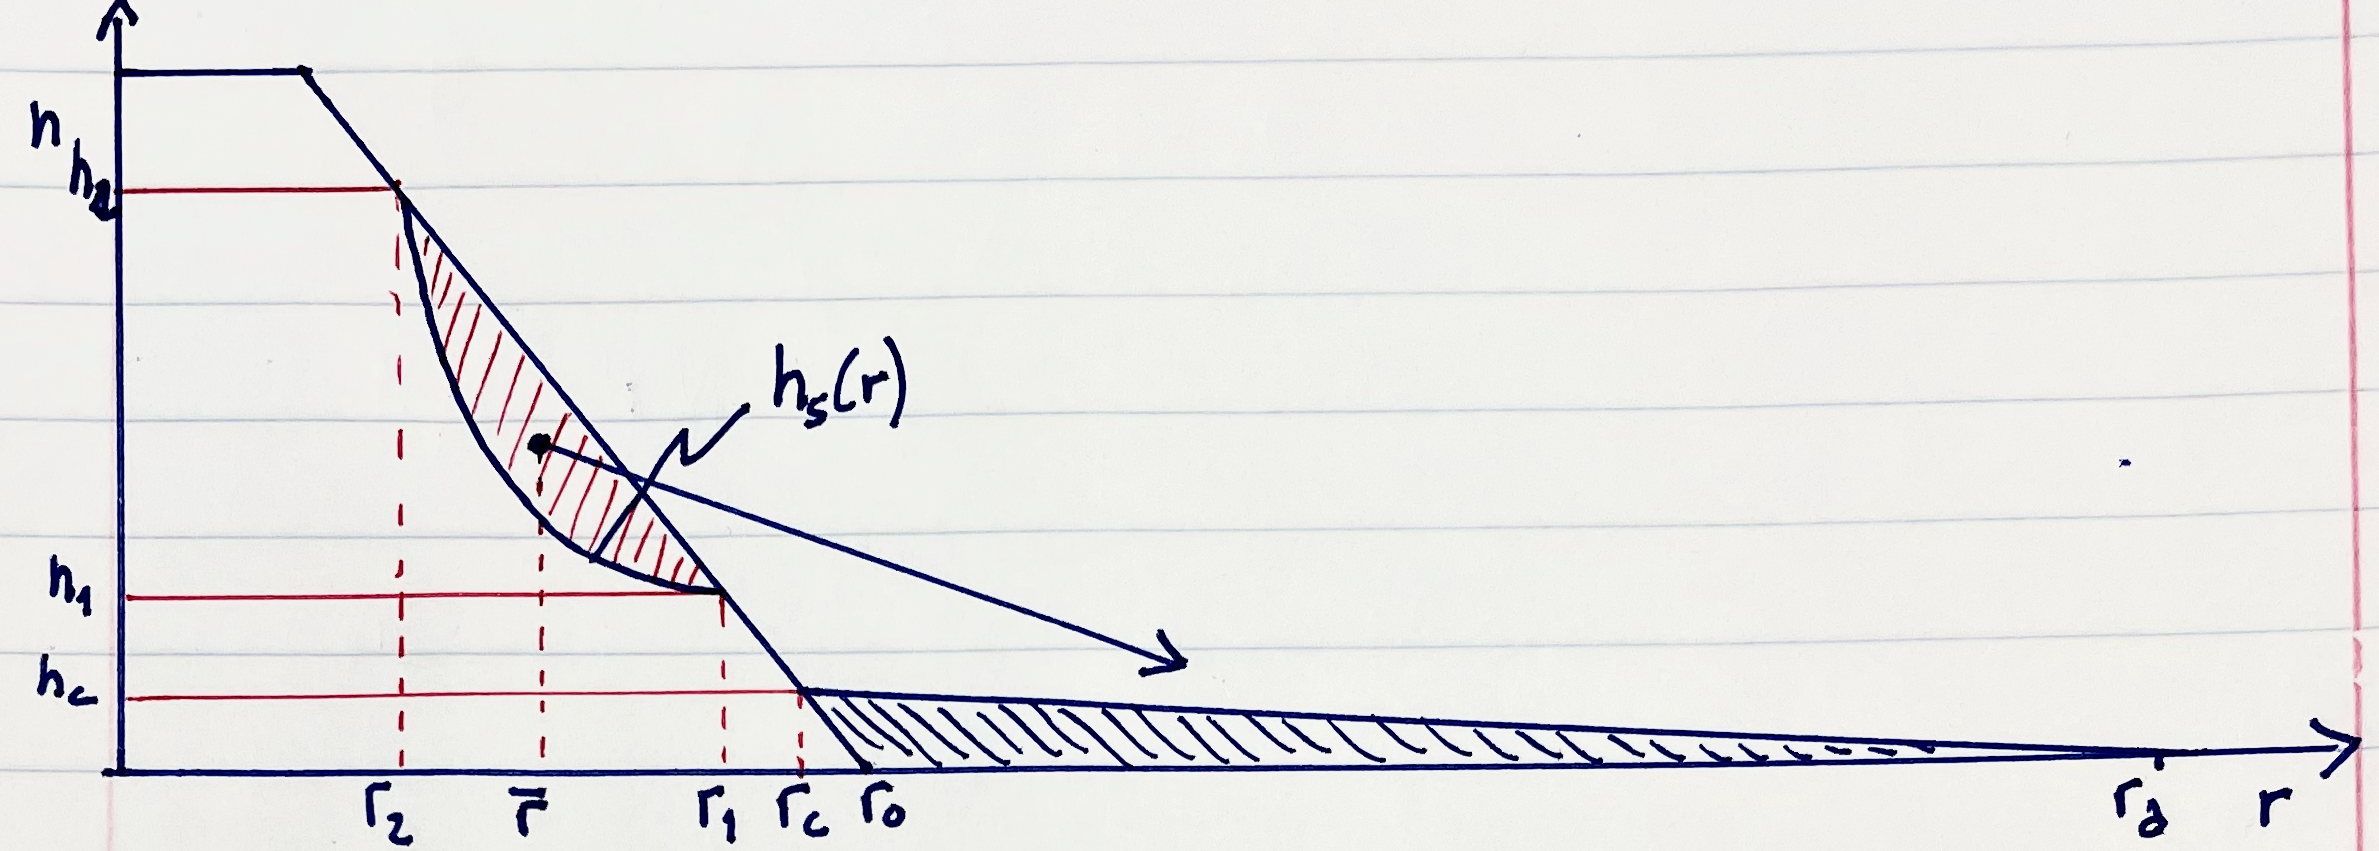
\includegraphics[width=\textwidth]{slides_fig1.png}
  \caption{Geometry for an ad-hoc landslide approximation in grdseamount.  The slide material (red hachured area)
  will be deposited at the toe of the seamount (blue hachured area) reaching up to a height of $h_c$ and linearly
  tapering to zero at a distal point $r_d$.}
  \label{slides_fig1}
\end{figure}

These notes resurrect the work of {\it J. Smith and Wessel} (2000) on approximating large landslides off seamounts
for the purpose of studying the isostatic consequences.  I found the old C codes and wanted to document the geometry
better as well as implement it as a new option in grdseamount.  I refer to Figure~\ref{slides_fig1}.  The equation for the
shape of the slide for the radial range $r_2$ to $r_1$ is given by a single equation:
\begin{equation}
h_s(r) = h_1 + \Delta h q(u),
\end{equation}
where $\Delta h = h_2 - h_1$ is the \emph{height} range of the slide and $q(u)$ is the normalized shape curve of the slide
modeled by
\begin{equation}
q(u) = u_0 \left (\frac{1 + u_0}{u + u_0} - 1 \right ).
\end{equation}
This is basically a hyperbolic curve and we can use the tuning parameter $u_0$ to carve more or less into the seamount core.
Here, $u$ is the normalized distance from $r_2$ to $r_1$ over which $q$ goes from 1 to 0:
\begin{equation}
u = \frac{r-r_2}{\Delta r},
\end{equation}
where $\Delta r = r_1 - r_2$ is the \emph{radial} range of the slide.
Figure~\ref{slides_fig2} shows the typical shapes of $q(u)$ for a range of $u_0$ values.
\begin{figure}[h!]
  \centering
  \includegraphics[width=\textwidth]{slides_fig2.png}
  \caption{A variety of slide shapes are possible by varying $u_0$.  The slide area for a conical seamount would be the area
  between the flank (dashed line) and the selected curve.}
  \label{slides_fig2}
\end{figure}

Depending on the shape of the seamount prior to the slide event (called $h(r)$), we will need to compute the various radii referred
to in Figure \ref{slides_fig1}, such as $r_1$, $r_2$, and $r_c$, from their corresponding heights $h_1$, $h_2, $ and $h_c$.
The material removed by the land slide (red hachured area)
will be deposited at the base of the seamount (blue hachured area) up to the proximal height $h_c$.  We assume this deposit will have a linearly
decaying height, enabling us to compute the distal radius $r_d$ from the volume of the slide, $V_s$.  Clearly $V_s$ depends
on both $h(r)$ and $h_s(r)$.  We will compute this volume as $V_s = V_f - V_q$, where $V_f$ is the flank volume whose
triangular (for a cone) crossection is delimited by the lines $r = r_2$, $h = h_1$ and $h(r)$.  Its area $A_f$ and centroid $\bar{r}_f$ are computed once and
we then use Pappas' theorem to get the corresponding volume $V_f = 2 \pi \bar{r}_f A_f$.  For $V_s$ the upper limit is $h_s(r)$ instead of $h(r)$ so we can integrate
$h_s(r)$ for an analytical answer. First we get the area:
\begin{equation}
A_s = \int_{r_2}^{r_1} h_s(r) dr = \Delta h \Delta r \int_0^1 q(u) du = \Delta h \Delta r \left \{ u_0 \left [ (1 + u_0) \log \left (\frac{1 + u_0}{u_0} \right ) - 1 \right ] \right \}.
\end{equation}
To use Pappas' theorem for computing the volume we need the radius to the centroid, which is obtained via
\begin{equation}
\bar{r} = \frac{\int_{r_2}^{r_1}h_s(r)rdr}{\int_{r_2}^{r_1}h_s(r)dr} = r_2 + \Delta r \bar{u} = r_2 + \Delta r \frac{\int_0^1q(u)udu}{\int_0^1 q(u)du}.
\end{equation}
This integral yields
\begin{equation}
\bar{u} = \frac{2(1 + u_0)\left [1 - u_0 \log \left ( \frac{1+u_0}{u_0} \right ) \right ] - 1}{(1 + u_0) \log \left (\frac{1 + u_0}{u_0} \right ) - 1}.
\end{equation}
Our final slide volume is therefore
\begin{equation}
V_s = V_f - 2 \pi \Delta h \Delta r \left ( r_2 + \Delta r\bar{u} \right ) u_0 \left [ (1 + u_0) \log \left (\frac{1 + u_0}{u_0} \right ) - 1 \right ].
\end{equation}
To solve for the distal end radius $r_d$ we need to equate the volume $V_s$ with the equivalent distal volume.
Given that the distal triangle area\footnote{We assume that $h(r)$ from $h_c$ to zero may be approximated as a linear ramp.} is
\begin{equation}
A_d = \frac{h_c}{2} (r_d - r_0),
\end{equation}
we find the volume to be
\begin{equation}
V_d = 2 \pi \bar{r}_d A_d = 2 \pi \bar{r}_d \left [ \frac{h_c}{2} (r_d - r_0) \right ],
\end{equation}
where $\bar{r}_d$ is the centroid radial distance of the distal triangle and is obtained in a similar fashion to $\bar{u}$ except
we must handle the awkward initial section separately:
\begin{equation}
\bar{r}_d = \frac{\int_{r_c}^{r_d}h_c \left (1 - \frac{r - r_c}{r_d - r_c} \right )rdr - \int_{r_c}^{r_o}h_c \left (1 - \frac{r - r_c}{r_o- r_c} \right )rdr}{A_d}
\end{equation}
Simplifying this expression and equating the two volumes lead to the quadratic equation
\begin{equation}
r_d^2 + r_c r_d - \left (r_0^2 - r_0 r_c + \frac{3 V_s}{\pi h_c}\right ) = r_d^2 + r_c r_d - c = 0,
\end{equation}
with unique solution
\begin{equation}
r_d = \frac{-r_c + \sqrt{r_c^2 + 4c}}{2}.
\end{equation}

It may be useful to state we want a slide that redeposits a fraction $\phi$ of the total volume $V_0$ of the entire seamount. In that
case we will need to compute $u_0$ given the other parameters to match the volumes.  We then have from above
\begin{equation}
V_s = \phi V_0 = V_f - 2 \pi \Delta h \Delta r \left ( r_2 + \Delta r\bar{u} \right ) u_0 \left [ (1 + u_0) \log \left (\frac{1 + u_0}{u_0} \right ) - 1 \right ].
\end{equation}
We rearrange this equation into the form
\begin{equation}
\left ( r_2 + \Delta r \bar{u} \right ) u_0 \left [ (1 + u_0) \log \left (\frac{1 + u_0}{u_0} \right ) - 1 \right ] = \frac{V_f - \phi V_0}{2 \pi \Delta h \Delta r}
\end{equation}
and solve for $u_0$ numerically.  We note that $V_s$ cannot exceed $V_f$ so $\phi$ is limited for the given other parameters.  As
$V_s$ pushes closer to $V_f$ we will get diminishing values for $u_0$.

Most slides do not involve the entire seamount, but instead affects a limited sector of it.  Thus, our slide sector is specified by two
azimuths $\alpha_1$ and $\alpha_2$ and the slide only affects that part of the seamount with a volume fraction
\begin{equation}
\theta = \frac{\alpha_2 - \alpha_1}{360}.
\end{equation}
In reporting volumes we need to scale by $\theta$ but the equations above balancing volumes are not affected since $\theta$ would cancel from both sides of the equations.

\section{REFERENCES}

Smith, J. R., and P. Wessel (2000), Isostatic consequences of giant landslides on the Hawaiian Ridge,
{\it ure Appl. Geophys., 157}, 1097--1114, doi:10.1007/s000240050019.
\end{document}
